\documentclass[11pt,a4paper]{article}

\usepackage[utf8]{inputenc}
\usepackage[T1]{fontenc}
\usepackage[spanish,provide=*]{babel}
\usepackage[margin=2.5cm]{geometry}
\usepackage{amsmath,amssymb}

\DeclareUnicodeCharacter{03B4}{\ensuremath{\delta}}
\DeclareUnicodeCharacter{03C3}{\ensuremath{\sigma}}
\DeclareUnicodeCharacter{03BB}{\ensuremath{\lambda}}
\DeclareUnicodeCharacter{221E}{\ensuremath{\infty}}
\DeclareUnicodeCharacter{222A}{\ensuremath{\cup}}
\DeclareUnicodeCharacter{00D7}{\ensuremath{\times}}
\DeclareUnicodeCharacter{2265}{\ensuremath{\ge}}
\DeclareUnicodeCharacter{2264}{\ensuremath{\le}}
\DeclareUnicodeCharacter{2260}{\ensuremath{\neq}}
\DeclareUnicodeCharacter{00AC}{\ensuremath{\lnot}}
\DeclareUnicodeCharacter{2227}{\ensuremath{\land}}
\DeclareUnicodeCharacter{2228}{\ensuremath{\lor}}
\DeclareUnicodeCharacter{2208}{\ensuremath{\in}}
\DeclareUnicodeCharacter{2192}{\ensuremath{\rightarrow}}
\DeclareUnicodeCharacter{2205}{\ensuremath{\emptyset}}
\DeclareUnicodeCharacter{2248}{\ensuremath{\approx}}

\usepackage{xcolor}
\usepackage{listings}
\usepackage{booktabs}
\usepackage{array}
\usepackage{enumitem}
\usepackage{tikz}
\usetikzlibrary{positioning,arrows.meta,fit,backgrounds,calc}
\usepackage{graphicx}
\usepackage{float}
\usepackage[hidelinks]{hyperref}

\setlist{nosep,leftmargin=1.4em}
\setlength{\emergencystretch}{3em}

\lstdefinestyle{cml}{
  basicstyle=\ttfamily\footnotesize,
  breaklines=true,
  breakautoindent=true,
  columns=fullflexible,
  keepspaces=true,
  frame=single,
  framesep=4pt,
  xleftmargin=2pt,
  rulecolor=\color{gray!45},
  backgroundcolor=\color{gray!5},
  extendedchars=true,
  literate=
    {δ}{{$\delta$}}1
    {σ}{{$\sigma$}}1
    {λ}{{$\lambda$}}1
    {∞}{{$\infty$}}1
    {∪}{{$\cup$}}1
    {×}{{$\times$}}1
    {≥}{{$\ge$}}1
    {≤}{{$\le$}}1
    {≠}{{$\neq$}}1
    {¬}{{$\lnot$\,}}1
    {∧}{{$\land$}}1
    {∨}{{$\lor$}}1
    {∈}{{$\in$}}1
    {→}{{$\rightarrow$}}1
    {∅}{{$\emptyset$}}1
    {≈}{{$\approx$}}1
    {á}{{\'a}}1 {é}{{\'e}}1 {í}{{\'i}}1 {ó}{{\'o}}1 {ú}{{\'u}}1
    {Á}{{\'A}}1 {É}{{\'E}}1 {Í}{{\'I}}1 {Ó}{{\'O}}1 {Ú}{{\'U}}1
    {ñ}{{\~n}}1 {Ñ}{{\~N}}1
}

\title{\textbf{Especificación DEVS}\\[2pt]
\large Controlador simplificado de una bomba de infusión}
\author{Juan Ignacio Villanueva \and Santiago Pesce}
\date{Simulación de Sistemas --- Departamento de Computación, Facultad de Ciencias Exactas, UNRC\\[2pt]
Junio de 2026}

\begin{document}
\maketitle

\begin{abstract}
\noindent
Modelamos en DEVS un controlador simplificado de una bomba de infusión intravenosa. El controlador recibe órdenes médicas, vigila el caudal real informado por un sensor contra el caudal indicado, detecta desvíos sostenidos, gestiona la condición de fin de bolsa y genera las alarmas correspondientes. Presentamos la especificación formal (estilo CML-DEVS) de los cinco modelos atómicos de dominio y del modelo acoplado, la implementación en Python con PyPDEVS —que suma tres componentes auxiliares: dos generadores estocásticos de eventos y un monitor observador— y la verificación de diez propiedades (de seguridad, vivacidad y temporales) sobre siete escenarios de simulación, todas sin violaciones.
\end{abstract}

\section{Descripción del sistema}

El sistema administra medicación intravenosa a un caudal indicado por una orden médica. En esta versión reducida nos concentramos en el controlador: recibe las órdenes, compara el caudal real (que el sensor informa cada segundo) contra el indicado y reacciona ante tres situaciones, desvíos sostenidos de caudal, fin de bolsa y alarmas críticas sin confirmar. El interés no está tanto en el control fino del caudal como en verificar que cada acción ocurra dentro de los tiempos especificados.

Modelamos el conjunto como un DEVS acoplado. El núcleo lo forman cinco componentes atómicos de dominio: un generador de órdenes, el controlador de bomba, el actuador, el sensor de flujo y un módulo de alarmas. El generador y el sensor son sencillos; el controlador concentra prácticamente toda la lógica, y el módulo de alarmas se encarga de la repetición de las alarmas críticas. A estos se suman tres componentes auxiliares de simulación (sección~\ref{sec:auxiliares}): dos generadores estocásticos —de fin de bolsa y de confirmación del enfermero— que producen los estímulos externos, y un monitor pasivo que recolecta las series y métricas usadas más tarde en la verificación.

\section{Interfaz y requisitos temporales}

El controlador recibe cuatro entradas: \texttt{ordenMedica} (caudal objetivo en ml/h, entre 0 y 200; un valor 0 detiene la infusión), \texttt{sensorFlujo} (caudal real medido), \texttt{finBolsa} (la bolsa está por agotarse) y \texttt{confirmacionEnfermero} (una alarma fue reconocida). Produce \texttt{ajustarCaudal}, \texttt{detenerBomba}, las alarmas \texttt{alarmaBaja}, \texttt{alarmaMedia} y \texttt{alarmaCritica}, y \texttt{registrarEvento} para la bitácora del sistema.

\begin{table}[h]
\centering
\small
\begin{tabular}{lr}
\toprule
Parámetro & Valor \\
\midrule
Rango de caudal permitido & 0 a 200 ml/h \\
Tiempo máximo para iniciar la infusión & 3 s \\
Período de muestreo del sensor & 1 s \\
Latencia del actuador & 0,5 s \\
Desvío máximo permitido de caudal & 10\% \\
Tiempo máximo de desvío tolerado & 5 s \\
Tiempo para confirmar una alarma crítica & 30 s \\
Período de repetición de la alarma crítica & 10 s \\
Tiempo máximo tras el fin de bolsa & 60 s \\
\bottomrule
\end{tabular}
\caption{Parámetros temporales del sistema.}
\end{table}

Los requisitos temporales que el modelo debe respetar son:

\begin{enumerate}
\item Tras una \texttt{ordenMedica} con caudal mayor que cero, la bomba debe iniciar la infusión en menos de 3 s.
\item La orden fija el caudal; la bomba lo mantiene hasta recibir una orden nueva. Caudal 0 detiene la infusión.
\item El sensor informa el caudal real cada 1 s.
\item Si el caudal real difiere más de 10\% del indicado durante más de 5 s, se emite \texttt{alarmaMedia}.
\item Si el desvío no se corrige tras la \texttt{alarmaMedia}, se escala a \texttt{alarmaCritica} y se detiene la bomba. El criterio exacto lo define cada grupo.
\item Si una \texttt{alarmaCritica} no se confirma en 30 s, debe repetirse cada 10 s.
\item Ante \texttt{finBolsa} se emite \texttt{alarmaBaja} y la infusión continúa como máximo 60 s, tras los cuales la bomba se detiene sola.
\item Después de una \texttt{alarmaCritica} la bomba queda detenida hasta recibir una \texttt{confirmacion\discretionary{}{}{}Enfermero} o una orden nueva.
\end{enumerate}

\section{Decisiones de modelado}\label{sec:decisiones}

Antes de las especificaciones conviene dejar claras las decisiones que tomamos, porque condicionan la lectura de las funciones de transición.

\paragraph{La salida sale siempre por $\lambda$.} En DEVS la salida se produce únicamente por la función $\lambda$, que se ejecuta antes de cada transición interna. Para emitir en respuesta a un evento de entrada usamos el patrón habitual: la transición externa no emite, sino que anota en una variable de estado qué corresponde emitir y agenda una transición interna inmediata ($\sigma = 0$); esa transición dispara $\lambda$ y luego $\delta_{int}$ deja el estado de reposo. En el controlador esa variable es \texttt{cmd}.

\paragraph{Desvío por conteo de muestras.} Como el sensor entrega una medición por segundo, en vez de un temporizador continuo para el desvío contamos muestras consecutivas fuera de tolerancia: 6 muestras equivalen a 6 s, cubriendo el ``más de 5 s'' del requisito. La sexta muestra dispara \texttt{alarmaMedia} y la novena escala a \texttt{alarmaCritica} (tres muestras más tras la media). Una muestra dentro de tolerancia reinicia el contador, lo que cubre de forma natural el caso del desvío leve que el controlador corrige a tiempo.

\paragraph{La repetición de la alarma crítica vive en el módulo de alarmas.} El requisito 6 (repetir cada 10 s una crítica sin confirmar) lo resuelve el módulo de alarmas, no el controlador. Así el controlador emite la crítica una sola vez y queda libre de ese temporizador, y la responsabilidad de insistir queda donde corresponde según el enunciado.

\paragraph{Criterio de escalamiento (requisito 5).} Definimos que el desvío debe persistir 3 s más después de la \texttt{alarmaMedia} (tres muestras adicionales) para escalar a \texttt{alarmaCritica} y detener la bomba. Esto da \texttt{N\_CRITICA = N\_MEDIA + 3 = 9}.

\paragraph{Durante el fin de bolsa no escalamos por desvío.} Una vez en modo \texttt{bolsa} ya se emitió la \texttt{alarmaBaja} y la bolsa se está agotando, así que dejamos que un único temporizador (la cuenta regresiva de 60 s) controle $\sigma$. Las muestras del sensor que llegan en ese intervalo solo actualizan el último valor medido y descuentan el tiempo transcurrido, sin disparar nuevas alarmas.

\section{Modelos atómicos}

Seguimos la notación de la tesis de Hollmann. Cada modelo declara únicamente las estructuras que usa, y $\sigma$ es la variable de estado cuyo valor devuelve la función de avance de tiempo $ta$.

\subsection{Generador de órdenes médicas}

Mantiene una agenda de órdenes, cada una con el caudal a indicar y el tiempo de espera hasta emitirla. No recibe eventos, así que omite $X$ y $\delta_{ext}$.

\begin{lstlisting}[style=cml]
atomic GenOrdenes is < Y, S, δint, λ, ta > where

Y is
  ordenMedica : R;              -- caudal objetivo (ml/h), 0 <= v <= 200
end Y

S is
  agenda : List (R × Time);     -- (caudal, espera hasta emitir)
  σ      : Time;
end S

δint((agenda, σ)) is
  defcases
    case s = (tail agenda, (head (tail agenda)).2);   if (#agenda > 1)
    case s = ({}, ∞);                                 if (#agenda ≤ 1)
  end defcases
end δint

λ((agenda, σ)) is
  ordenMedica = (head agenda).1;
end λ

ta((agenda, σ)) is
  σ;
end ta

end atomic
\end{lstlisting}

\noindent Estado inicial: \texttt{agenda} con el escenario a simular y \texttt{σ = (head agenda).2}. Para un escenario estocástico se llena la agenda con caudales y tiempos generados a partir de las distribuciones elegidas; la estructura del modelo no cambia.

\subsection{Sensor de flujo}

Mide el caudal real y lo informa cada segundo. Una medición nueva del actuador no reinicia el período de muestreo: solo actualiza el valor retenido.

\begin{lstlisting}[style=cml]
P is
  T_muestreo = 1;               -- periodo de muestreo (s)
end P

atomic SensorFlujo is < X, Y, S, δint, δext, λ, ta > where

X is
  caudalActual : R;
end X

Y is
  sensorFlujo : R;
end Y

S is
  caudal : R;                   -- ultimo caudal real informado
  σ      : Time;
end S

δint((caudal, σ)) is
  σ = T_muestreo;               -- rearma el periodo completo
end δint

δext((caudal, σ), e, (caudalActual, value)) is
  caudal = value;
  σ = σ - e;                    -- no reinicia: solo descuenta lo transcurrido
end δext

λ((caudal, σ)) is
  sensorFlujo = caudal;
end λ

ta((caudal, σ)) is
  σ;
end ta

end atomic
\end{lstlisting}

\noindent Estado inicial: \texttt{(0, T\_muestreo)}.

\subsection{Actuador de la bomba}

Recibe órdenes del controlador y aplica el caudal con una latencia de 0,5 s. Al aplicarlo informa el nuevo caudal real.

\begin{lstlisting}[style=cml]
P is
  T_latencia = 0.5;             -- latencia del actuador (s)
end P

atomic Actuador is < X, Y, S, δint, δext, λ, ta > where

X is
  ajustarCaudal : R;
  detenerBomba  : {stop};
end X

Y is
  caudalActual : R;
end Y

S is
  objetivo : R;                 -- caudal a aplicar tras la latencia
  σ        : Time;
end S

δext((objetivo, σ), e, (port, value)) is
  defcases
    case s = (value, T_latencia);   if (port = ajustarCaudal)
    case s = (0,     T_latencia);   if (port = detenerBomba)
  end defcases
end δext

δint((objetivo, σ)) is
  σ = ∞;                        -- aplicado; pasivo hasta nueva orden
end δint

λ((objetivo, σ)) is
  caudalActual = objetivo;
end λ

ta((objetivo, σ)) is
  σ;
end ta

end atomic
\end{lstlisting}

\noindent Estado inicial: \texttt{(0, ∞)}.

\subsection{Controlador de bomba}

Es el núcleo del sistema. Funciona como una máquina de estados con cuatro modos: \texttt{idle} (sin infusión), \texttt{infund} (infundiendo y vigilando), \texttt{bolsa} (fin de bolsa, con cuenta regresiva de 60 s) y \texttt{detenida} (frenada tras una crítica, a la espera de confirmación u orden nueva). La variable \texttt{cmd} indica qué debe emitir la próxima transición interna, según el patrón descrito en la sección~\ref{sec:decisiones}. La función auxiliar \texttt{desviado} decide si una medición está fuera de tolerancia.

\begin{lstlisting}[style=cml]
P is
  MAX_CAUDAL = 200;             -- ml/h
  TOL        = 0.10;            -- 10%
  N_MEDIA    = 6;               -- muestras consecutivas para alarmaMedia (> 5 s)
  N_CRITICA  = 9;               -- N_MEDIA + 3 -> alarmaCritica (3 s despues)
  T_BOLSA    = 60;              -- ventana maxima tras fin de bolsa (s)
end P

functions
  function desviado is
    real : R, obj : R → res : Boolean;
    res = ( max(real - obj, obj - real) > TOL * obj );
  end function
end functions

atomic Controlador is < X, Y, S, δint, δext, λ, ta > where

X is
  ordenMedica           : R;
  sensorFlujo           : R;
  finBolsa              : {signal};
  confirmacionEnfermero : {signal};
end X

Y is
  ajustarCaudal   : R;
  detenerBomba    : {stop};
  alarmaBaja      : {signal};
  alarmaMedia     : {signal};
  alarmaCritica   : {signal};
  registrarEvento : Text;
end Y

S is
  Cmd == {nada, iniciar, parar, corregir, media, critica, baja, autostop, confirmar, reanudar};
  modo     : {idle, infund, bolsa, detenida};
  objetivo : R;                 -- caudal ordenado vigente
  medido   : R;                 -- ultima medicion del sensor
  desvios  : N;                 -- muestras consecutivas con desvio
  cmd      : Cmd;               -- que emitir en la proxima transicion interna
  σ        : Time;
end S

δext((modo, objetivo, medido, desvios, cmd, σ), e, (port, value)) is
  defcases
    -- Orden medica (valida en cualquier modo)
    case s = (infund, value, medido, 0, iniciar, 0);
         if ((port = ordenMedica) ∧ (value > 0))
    case s = (idle, 0, medido, 0, parar, 0);
         if ((port = ordenMedica) ∧ (value = 0))

    -- Fin de bolsa (solo si esta infundiendo)
    case s = (bolsa, objetivo, medido, desvios, baja, 0);
         if ((port = finBolsa) ∧ (modo = infund))

    -- Confirmacion del enfermero
    case s = (idle, 0, medido, 0, confirmar, 0);           -- libera el bloqueo posterior a una critica
         if ((port = confirmacionEnfermero) ∧ (modo = detenida))
    case s = (infund, objetivo, medido, 0, reanudar, 0);   -- cambio de bolsa: reanuda la infusion
         if ((port = confirmacionEnfermero) ∧ (modo = bolsa))

    -- Sensor de flujo durante infusion: deteccion y escalamiento por desvio
    case s = (detenida, objetivo, value, desvios + 1, critica, 0);
         if ((port = sensorFlujo) ∧ (modo = infund) ∧ desviado(value, objetivo) ∧ (desvios + 1 ≥ N_CRITICA))
    case s = (infund, objetivo, value, desvios + 1, media, 0);
         if ((port = sensorFlujo) ∧ (modo = infund) ∧ desviado(value, objetivo) ∧ (desvios + 1 = N_MEDIA))
    case s = (infund, objetivo, value, desvios + 1, nada, ∞);   -- entre media y critica: cuenta sin reordenar
         if ((port = sensorFlujo) ∧ (modo = infund) ∧ desviado(value, objetivo) ∧ (desvios + 1 > N_MEDIA))
    case s = (infund, objetivo, value, desvios + 1, corregir, 0);   -- desvio leve aun corregible
         if ((port = sensorFlujo) ∧ (modo = infund) ∧ desviado(value, objetivo))
    case s = (infund, objetivo, value, 0, nada, ∞);            -- vuelve a tolerancia: reinicia el contador
         if ((port = sensorFlujo) ∧ (modo = infund) ∧ ¬ desviado(value, objetivo))

    -- Sensor durante fin de bolsa: solo registra, conserva la cuenta regresiva
    case s = (bolsa, objetivo, value, desvios, cmd, σ - e);
         if ((port = sensorFlujo) ∧ (modo = bolsa))

    -- Evento que no aplica al modo actual (incluida una confirmacion en idle/infund): se ignora
    default s = (modo, objetivo, medido, desvios, cmd, σ - e);
  end defcases
end δext

δint((modo, objetivo, medido, desvios, cmd, σ)) is
  defcases
    case s = (infund,   objetivo, medido, desvios, nada,     ∞);        if (cmd = iniciar)
    case s = (idle,     0,        medido, 0,       nada,     ∞);        if (cmd = parar)
    case s = (infund,   objetivo, medido, desvios, nada,     ∞);        if (cmd = corregir)
    case s = (infund,   objetivo, medido, desvios, nada,     ∞);        if (cmd = media)
    case s = (detenida, objetivo, medido, 0,       nada,     ∞);        if (cmd = critica)
    case s = (bolsa,    objetivo, medido, desvios, autostop, T_BOLSA);  if (cmd = baja)
    case s = (idle,     0,        medido, 0,       nada,     ∞);        if (cmd = autostop)
    case s = (idle,     0,        medido, 0,       nada,     ∞);        if (cmd = confirmar)
    case s = (infund,   objetivo, medido, desvios, nada,     ∞);        if (cmd = reanudar)
    default s = (modo, objetivo, medido, desvios, nada, ∞);
  end defcases
end δint

λ((modo, objetivo, medido, desvios, cmd, σ)) is
  defcases
    case ajustarCaudal = objetivo, registrarEvento = "inicio_infusion";              if (cmd = iniciar)
    case detenerBomba  = stop,     registrarEvento = "stop_por_orden";               if (cmd = parar)
    case ajustarCaudal = objetivo, registrarEvento = "correccion_caudal";            if (cmd = corregir)
    case alarmaMedia   = signal,   registrarEvento = "desvio_sostenido";             if (cmd = media)
    case alarmaCritica = signal, detenerBomba = stop, registrarEvento = "critica_stop";   if (cmd = critica)
    case alarmaBaja    = signal,   registrarEvento = "fin_bolsa";                     if (cmd = baja)
    case detenerBomba  = stop,     registrarEvento = "autostop_fin_bolsa";            if (cmd = autostop)
    case registrarEvento = "confirmacion_enfermero";                                  if (cmd = confirmar)
    case ajustarCaudal = objetivo, registrarEvento = "reanudacion_post_bolsa";        if (cmd = reanudar)
  end defcases
end λ

ta((modo, objetivo, medido, desvios, cmd, σ)) is
  σ;
end ta

end atomic
\end{lstlisting}

\noindent Estado inicial: \texttt{(idle, 0, 0, 0, nada, ∞)}.

La secuencia de fin de bolsa muestra cómo cooperan $\sigma$ y \texttt{cmd}: la transición externa fija \texttt{cmd = baja} y $\sigma = 0$; $\lambda$ emite la \texttt{alarmaBaja}; la transición interna del caso \texttt{baja} deja \texttt{cmd = autostop} y $\sigma = 60$. Durante esos 60 s las muestras del sensor solo descuentan $\sigma$, de modo que cuando llega a cero la transición interna dispara con \texttt{cmd = autostop} y detiene la bomba. Si en cambio durante esa ventana llega una \texttt{confirmacion\-Enfermero} (el enfermero repuso la bolsa), la transición externa fija \texttt{cmd = reanudar} y $\sigma = 0$: $\lambda$ vuelve a ordenar el caudal vigente (\texttt{reanudacion\_post\_bolsa}), el modo regresa a \texttt{infund} y el \texttt{autostop} queda cancelado.

\paragraph{El conteo no reordena entre la media y la crítica.} Una vez emitida la \texttt{alarmaMedia} (sexta muestra desviada), las muestras 7 y 8 que sigan fuera de tolerancia ya no emiten \texttt{correccion\_caudal}: solo incrementan el contador con \texttt{cmd = nada} (de ahí el caso \texttt{desvios + 1 > N\_MEDIA} en $\delta_{ext}$). El sistema ya avisó del desvío sostenido y está a la espera de ver si escala; insistir con la misma orden de caudal no aportaría nada hasta que la novena muestra dispare la \texttt{alarmaCritica}.

\subsection{Módulo de alarmas}

Gestiona las notificaciones. Las alarmas \texttt{baja} y \texttt{media} suenan una vez. La crítica insiste: si no se confirma en 30 s vuelve a sonar y luego se repite cada 10 s hasta la confirmación.

\begin{lstlisting}[style=cml]
P is
  T_CONF = 30;                  -- espera inicial de confirmacion (s)
  T_REP  = 10;                  -- periodo de repeticion (s)
end P

atomic ModuloAlarmas is < X, Y, S, δint, δext, λ, ta > where

X is
  alarmaBaja            : {signal};
  alarmaMedia           : {signal};
  alarmaCritica         : {signal};
  confirmacionEnfermero : {signal};
end X

Y is
  notificacionAlarma : Text;
end Y

S is
  modo : {ocioso, critInic, esperaConf, repitiendo};
  pend : Text ∪ {∅};            -- mensaje a emitir en la proxima interna
  σ    : Time;
end S

δext((modo, pend, σ), e, (port, value)) is
  defcases
    case s = (ocioso,   "baja",    0);     if (port = alarmaBaja)
    case s = (ocioso,   "media",   0);     if (port = alarmaMedia)
    case s = (critInic, "critica", 0);     if ((port = alarmaCritica) ∧ (modo = ocioso))
    case s = (ocioso,   ∅,         ∞);     if (port = confirmacionEnfermero)
    default s = (modo, pend, σ - e);
  end defcases
end δext

δint((modo, pend, σ)) is
  defcases
    case s = (ocioso,     ∅,         ∞);       if (modo = ocioso)
    case s = (esperaConf, "critica", T_CONF);  if (modo = critInic)
    case s = (repitiendo, "critica", T_REP);   if (modo = esperaConf)
    case s = (repitiendo, "critica", T_REP);   if (modo = repitiendo)
  end defcases
end δint

λ((modo, pend, σ)) is
  notificacionAlarma = pend;
end λ

ta((modo, pend, σ)) is
  σ;
end ta

end atomic
\end{lstlisting}

\noindent Estado inicial: \texttt{(ocioso, ∅, ∞)}.

\subsection{Componentes auxiliares}\label{sec:auxiliares}

Los cinco modelos anteriores son el núcleo del sistema. Para cerrar el banco de simulación —generar los estímulos externos y recolectar los resultados— el modelo acoplado incorpora tres componentes atómicos auxiliares más. No agregan lógica de control, así que no detallamos su especificación CML completa, pero conviene describirlos porque aparecen en el acoplado de la sección siguiente.

\begin{itemize}
  \item \textbf{Generador de fin de bolsa} (\texttt{GenAlarmaFinBolsa}): emite la señal \texttt{finBolsa} una sola vez por corrida, en un instante aleatorio con distribución exponencial de media configurable (una sola bolsa por simulación). Tras emitir, queda pasivo ($\sigma = \infty$).
  \item \textbf{Generador de confirmación} (\texttt{GenConfirmacionEnfermero}): modela las rondas del enfermero. Emite \texttt{confirmacionEnfermero} en instantes aleatorios y se reprograma con una nueva muestra exponencial tras cada emisión. El evento solo tiene efecto si hay una situación que confirmar (alarma crítica activa o fin de bolsa en curso); en otro caso el controlador y el módulo de alarmas lo ignoran.
  \item \textbf{Monitor} (\texttt{Monitor}): observador pasivo. Recibe \texttt{ajustarCaudal}, \texttt{caudalActual}, \texttt{sensorFlujo}, \texttt{registrarEvento} y \texttt{notificacionAlarma}, pero no produce ninguna salida ($ta \equiv \infty$): solo registra las series temporales y calcula las métricas que se usan en la verificación de propiedades y en los resultados (secciones~\ref{sec:propiedades} y~\ref{sec:resultados}). Reconstruye el modo de la bomba de forma determinista a partir de la traza de \texttt{registrarEvento}, sin tocar la lógica del controlador.
\end{itemize}

\noindent Tanto los generadores como el monitor reciben una \emph{semilla} opcional para reproducibilidad. Los generadores pueden quedar desactivados ($\text{media} = \infty$) cuando un escenario prefiere inyectar \texttt{finBolsa} o \texttt{confirmacionEnfermero} en instantes fijos a través de las entradas externas del acoplado.

\section{Modelo acoplado}

El acoplado $N$ conecta los ocho componentes: los cinco de dominio y los tres auxiliares de la sección~\ref{sec:auxiliares}. Las señales \texttt{finBolsa} y \texttt{confirmacionEnfermero} las producen los generadores internos \texttt{GenFB} y \texttt{GenCF}; además se conservan como entradas externas de $N$ (EIC), como vía alternativa para forzar un evento puntual desde un escenario en un instante fijo, sin depender del azar de los generadores. Las salidas \texttt{sensorFlujo} y \texttt{caudalActual} se exponen para graficar y, junto con \texttt{registrarEvento} y \texttt{notificacionAlarma}, las observa internamente el \texttt{Monitor}.

\begin{lstlisting}[style=cml]
N = < X_N, Y_N, D, {M_d}, EIC, EOC, IC, Select >

X_N = { finBolsa : {signal},  confirmacionEnfermero : {signal} }
Y_N = { registrarEvento : Text,  notificacionAlarma : Text,
        sensorFlujo : R,  caudalActual : R }

D = { G, GenFB, GenCF, Sen, Ctrl, Act, Alm, Mon }
M_G     = GenOrdenes              M_GenFB = GenAlarmaFinBolsa
M_GenCF = GenConfirmacionEnfermero    M_Sen = SensorFlujo
M_Ctrl  = Controlador             M_Act = Actuador
M_Alm   = ModuloAlarmas           M_Mon = Monitor

EIC = {                                    -- entradas externas de N (via alternativa
                                           --   a los generadores internos GenFB / GenCF)
  [(N, finBolsa),              (Ctrl, finBolsa)],
  [(N, confirmacionEnfermero), (Ctrl, confirmacionEnfermero)],
  [(N, confirmacionEnfermero), (Alm,  confirmacionEnfermero)]
}

IC = {                                     -- conexiones internas
  [(G,     ordenMedica),           (Ctrl, ordenMedica)],
  [(GenFB, finBolsa),              (Ctrl, finBolsa)],
  [(GenCF, confirmacionEnfermero), (Ctrl, confirmacionEnfermero)],
  [(GenCF, confirmacionEnfermero), (Alm,  confirmacionEnfermero)],
  [(Sen,   sensorFlujo),           (Ctrl, sensorFlujo)],
  [(Ctrl,  ajustarCaudal),         (Act,  ajustarCaudal)],
  [(Ctrl,  detenerBomba),          (Act,  detenerBomba)],
  [(Act,   caudalActual),          (Sen,  caudalActual)],
  [(Ctrl,  alarmaBaja),            (Alm,  alarmaBaja)],
  [(Ctrl,  alarmaMedia),           (Alm,  alarmaMedia)],
  [(Ctrl,  alarmaCritica),         (Alm,  alarmaCritica)],
  -- observacion del Monitor (no realimenta el control)
  [(Ctrl,  ajustarCaudal),         (Mon,  ajustarCaudal)],
  [(Act,   caudalActual),          (Mon,  caudalActual)],
  [(Sen,   sensorFlujo),           (Mon,  sensorFlujo)],
  [(Ctrl,  registrarEvento),       (Mon,  registrarEvento)],
  [(Alm,   notificacionAlarma),    (Mon,  notificacionAlarma)]
}

EOC = {                                    -- componentes hacia salidas de N
  [(Ctrl, registrarEvento),    (N, registrarEvento)],
  [(Alm,  notificacionAlarma), (N, notificacionAlarma)],
  [(Sen,  sensorFlujo),        (N, sensorFlujo)],
  [(Act,  caudalActual),       (N, caudalActual)]
}

Select = < Ctrl, Act, Sen, Alm, Mon, G, GenFB, GenCF >   -- prioridad ante empates
\end{lstlisting}

El corazón del modelo es el lazo de control \texttt{Ctrl} $\rightarrow$ \texttt{Act} $\rightarrow$ \texttt{Sen} $\rightarrow$ \texttt{Ctrl}: el controlador ordena el caudal, el actuador lo aplica con su latencia, el sensor lo mide y se lo devuelve al controlador. La función \texttt{Select} da prioridad al controlador cuando dos transiciones internas caen en el mismo instante, de modo que la decisión se toma antes de propagar sus efectos; el \texttt{Monitor} se ubica entre los receptores reactivos (antes que los generadores) para registrar cada salida en el mismo instante en que se produce. La figura~\ref{fig:acoplado} muestra el modelo completo.

\begin{figure}[h]
\centering
\resizebox{\textwidth}{!}{%
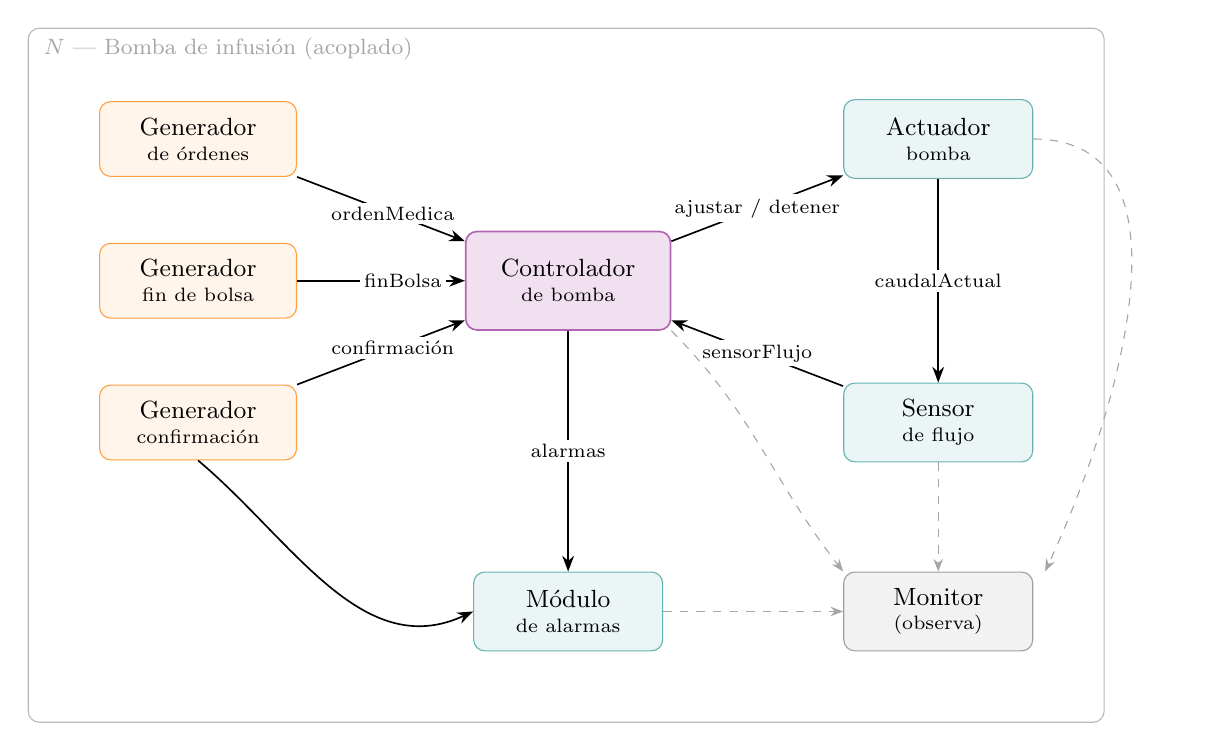
\begin{tikzpicture}[
  font=\small,
  comp/.style={draw=teal!60, rounded corners, minimum width=2.4cm, minimum height=1.0cm, align=center, fill=teal!8},
  gens/.style={draw=orange!75, rounded corners, minimum width=2.5cm, minimum height=0.95cm, align=center, fill=orange!8},
  hub/.style={draw=violet!60, rounded corners, minimum width=2.6cm, minimum height=1.25cm, align=center, fill=violet!12, line width=0.6pt},
  obs/.style={draw=gray!75, rounded corners, minimum width=2.4cm, minimum height=1.0cm, align=center, fill=gray!10},
  ic/.style={-{Stealth[length=2mm]}, semithick},
  tap/.style={-{Stealth[length=1.6mm]}, thin, dashed, draw=gray!70},
  lbl/.style={font=\scriptsize, fill=white, inner sep=1.5pt},
  elbl/.style={font=\scriptsize, inner sep=1.5pt}
]
% Generadores (fuentes, izquierda)
\node[gens] (gord) at (0,4.4)  {Generador\\[-2pt]\scriptsize de órdenes};
\node[gens] (gfb)  at (0,2.6)  {Generador\\[-2pt]\scriptsize fin de bolsa};
\node[gens] (gcf)  at (0,0.8)  {Generador\\[-2pt]\scriptsize confirmación};
% Lazo de control
\node[hub]  (ctrl) at (4.7,2.6)  {Controlador\\[-2pt]\scriptsize de bomba};
\node[comp] (act)  at (9.4,4.4)  {Actuador\\[-2pt]\scriptsize bomba};
\node[comp] (sen)  at (9.4,0.8)  {Sensor\\[-2pt]\scriptsize de flujo};
\node[comp] (alm)  at (4.7,-1.6) {Módulo\\[-2pt]\scriptsize de alarmas};
% Observador
\node[obs]  (mon)  at (9.4,-1.6) {Monitor\\[-2pt]\scriptsize (observa)};

\begin{scope}[on background layer]
  \node[draw=gray!55, rounded corners, fit=(gord)(gfb)(gcf)(ctrl)(act)(sen)(alm)(mon), inner sep=9mm] (N) {};
  \node[anchor=north west, gray!70, font=\footnotesize] at (N.north west) {\;$N$ --- Bomba de infusión (acoplado)};
\end{scope}

% Acoplamientos internos (IC) del lazo de control
\draw[ic] (gord) -- (ctrl) node[lbl,pos=0.57]{ordenMedica};
\draw[ic] (gfb)  -- (ctrl) node[lbl,pos=0.63]{finBolsa};
\draw[ic] (gcf)  -- (ctrl) node[lbl,pos=0.57]{confirmación};
\draw[ic] (gcf.south) to[out=-40,in=205] (alm.west);
\draw[ic] (ctrl) -- (act)  node[lbl,pos=0.5]{ajustar / detener};
\draw[ic] (act)  -- (sen)  node[lbl,pos=0.5]{caudalActual};
\draw[ic] (sen)  -- (ctrl) node[lbl,pos=0.5]{sensorFlujo};
\draw[ic] (ctrl) -- (alm)  node[lbl,pos=0.5]{alarmas};

% Observación del Monitor (punteada: no realimenta el control)
\draw[tap] (ctrl.south east) to[out=-45,in=128] (mon.north west);
\draw[tap] (act.east) to[out=0,in=65] ($(mon.north east)+(0.15,0)$);
\draw[tap] (sen.south) -- (mon.north);
\draw[tap] (alm.east) -- (mon.west);
\end{tikzpicture}%
}
\caption{Modelo acoplado $N$ con sus ocho componentes. Líneas sólidas: acoplamientos internos de control (IC). Líneas punteadas: el \emph{Monitor} observa las salidas relevantes (\texttt{ajustarCaudal}, \texttt{caudalActual}, \texttt{sensorFlujo}, \texttt{registrarEvento}, \texttt{notificacionAlarma}) sin realimentar el lazo. Las señales \texttt{finBolsa} y \texttt{confirmación} las producen los generadores internos y también pueden inyectarse desde fuera de $N$ (EIC); $N$ expone además \texttt{registrarEvento}, \texttt{notificacionAlarma}, \texttt{sensorFlujo} y \texttt{caudalActual} como salidas (EOC).}
\label{fig:acoplado}
\end{figure}

\section{Cumplimiento de los requisitos}

\begin{table}[h]
\centering
\small
\renewcommand{\arraystretch}{1.15}
\begin{tabular}{>{\raggedright}p{1.2cm} p{12.5cm}}
\toprule
Req. & Dónde se cumple \\
\midrule
1 & \texttt{Ctrl} emite \texttt{ajustarCaudal} en $\sigma = 0$, más 0,5 s de latencia del actuador: muy por debajo de 3 s. \\
2 & \texttt{objetivo} persiste hasta una orden nueva; el caso \texttt{ordenMedica = 0} lleva a \texttt{idle}. \\
3 & \texttt{SensorFlujo} con \texttt{T\_muestreo = 1}. \\
4 & Conteo de \texttt{N\_MEDIA = 6} muestras consecutivas fuera de tolerancia (cubre ``más de 5~s''). \\
5 & Escalamiento a \texttt{N\_CRITICA = 9} muestras (tres más tras la media, 3~s adicionales). \\
6 & \texttt{ModuloAlarmas}: espera 30 s y luego repite cada 10 s. \\
7 & Modo \texttt{bolsa}: emite \texttt{alarmaBaja}; la cuenta de 60~s termina en \texttt{autostop}, salvo que una confirmación reanude la infusión antes (\texttt{reanudar}). \\
8 & Modo \texttt{detenida}: solo sale por confirmación o por una orden nueva. \\
9.1 & En \texttt{idle} y \texttt{detenida} no se emite \texttt{ajustarCaudal}; las órdenes están acotadas a 0--200 ml/h. \\
\bottomrule
\end{tabular}
\caption{Trazabilidad entre requisitos y especificación.}
\end{table}

Los requisitos 1--8 se verifican en los escenarios de simulación de la sección~\ref{sec:resultados}.

\section{Implementación}

Los modelos se implementaron en Python~3 usando PyPDEVS (simulador clásico DEVS). Cada modelo atómico es una subclase de \texttt{AtomicDEVS} con los métodos \texttt{timeAdvance}, \texttt{outputFnc}, \texttt{intTransition} y \texttt{extTransition}. El estado es un objeto Python mutable; las transiciones lo modifican in place y lo retornan. El código se reparte en \texttt{modelos.py} (los ocho modelos atómicos y el acoplado), \texttt{escenarios.py} (los siete escenarios y la corrida), \texttt{propiedades.py} (verificador de propiedades) y \texttt{graficos.py} (gráficos y métricas).

\paragraph{Herramientas.} Python~3.14, PyPDEVS (Classic DEVS, instalado desde un fork compatible con Python~3, ya que el original quedó en Python~2) y \texttt{matplotlib} para los gráficos. El módulo \texttt{compat.py} reescribe \texttt{RootDEVS.setScheduler} para instanciar el scheduler con \texttt{importlib}, en vez del \texttt{exec}+\texttt{eval} del fork que dejó de funcionar en Python~3.13 (cambio de semántica de \texttt{locals()}/\texttt{exec}, PEP~667). De forma independiente, la clase base \texttt{Atomico} define \texttt{\_\_lt\_\_} (orden por nombre): el solver clásico ordena la lista de modelos inminentes cuando hay más de uno a la vez, y los objetos Python no son comparables por defecto.

\paragraph{Decisiones de implementación.}
\begin{itemize}
  \item El estado del controlador incluye \texttt{cmd} (qué emitir en la próxima \texttt{intTransition}) para reproducir exactamente el patrón $\lambda$-antes-de-$\delta_{int}$ de la especificación.
  \item El actuador acepta un parámetro \texttt{falla} ($\in (0,1]$) que escala el caudal entregado, permitiendo inyectar desvíos de forma controlada en los escenarios.
  \item Los generadores de fin de bolsa y de confirmación toman muestras exponenciales (\texttt{random.expovariate}) con media y semilla configurables; con media~$=\infty$ quedan inertes, para escenarios determinísticos que prefieren inyectar esos eventos en instantes fijos.
  \item El \texttt{Monitor} no expone puertos de salida ($ta \equiv \infty$): solo observa. Reconstruye el modo de la bomba de forma determinista a partir de la traza de \texttt{registrarEvento} (cada string mapea uno a uno con una transición de modo conocida), de modo que recolectar resultados no exige tocar la lógica del controlador.
  \item \texttt{ModuloAlarmas.extTransition} para \texttt{confirmacionEnfermero} verifica si $\sigma = 0$ antes de cancelar: si hay una transición interna inminente, PyPDEVS le da prioridad; la confirmación que llega en ese instante se procesa en el paso siguiente. Esto evita silenciar una notificación ya programada.
  \item Todos los descuentos de $\sigma$ en transiciones externas usan \texttt{max(0, σ - elapsed)} para evitar valores negativos por errores de punto flotante.
\end{itemize}

\paragraph{Escenarios y verificación.} Se definen en \texttt{escenarios.py}. Cada escenario arma el acoplado con su agenda de órdenes y, opcionalmente, un \texttt{Disparador} que inyecta \texttt{finBolsa} o \texttt{confirmacionEnfermero} en instantes fijos a través de las entradas externas de $N$; un \texttt{Registro} captura con marca de tiempo las salidas para imprimir la traza. Al terminar la corrida, \texttt{graficos.py} produce los gráficos y métricas a partir del estado final del \texttt{Monitor}, y \texttt{propiedades.py} corre sobre esa misma traza las diez verificaciones de la sección~\ref{sec:propiedades}.

\section{Propiedades a verificar}\label{sec:propiedades}

Más allá de la trazabilidad del cuadro anterior, fijamos un conjunto de propiedades que el sistema debe cumplir y las verificamos de forma automática. El verificador (\texttt{propiedades.py}) corre sobre la traza que el \texttt{Monitor} registró durante cada simulación y devuelve, por propiedad, \textsc{pasa}, \textsc{falla} o \textsc{n/a} (no aplica en ese escenario; por ejemplo, evaluar la repetición de una alarma crítica cuando nunca hubo una).

\paragraph{Verificación no tautológica.} Cada chequeo se construyó para \emph{no} depender de las constantes del código (\texttt{T\_LATENCIA}, \texttt{T\_BOLSA}, etc.): contrastar contra esas constantes solo confirmaría que están bien escritas, no que el sistema se comporta como debe. En su lugar miden el tiempo real transcurrido entre el evento causa y el evento efecto sobre los datos efectivamente simulados (instantes de \texttt{ordenMedica}, primer cambio del caudal real, instantes de \texttt{alarmaMedia}/\texttt{alarmaCritica}, de \texttt{finBolsa} y de su resolución).

Las diez propiedades se agrupan en tres categorías.

\paragraph{Seguridad (safety) --- ``nada incorrecto ocurre''.}
\begin{enumerate}[label=\textbf{S\arabic*.},leftmargin=2.6em]
  \item La bomba no administra caudal mientras la última orden recibida indique 0.
  \item El caudal real nunca supera el máximo permitido (200~ml/h).
  \item Tras una \texttt{alarmaCritica}, la bomba no reanuda la infusión hasta una confirmación o una orden nueva.
\end{enumerate}

\paragraph{Vivacidad (liveness) --- ``algo correcto ocurre eventualmente''.}
\begin{enumerate}[label=\textbf{L\arabic*.},leftmargin=2.6em]
  \item Toda orden médica produce eventualmente una acción efectiva sobre el caudal real, no solo el registro del evento.
  \item Toda \texttt{alarmaCritica} no confirmada se repite eventualmente.
  \item Todo \texttt{finBolsa} se resuelve eventualmente (autostop, reanudación o nueva orden).
\end{enumerate}

\paragraph{Temporales --- los plazos del enunciado.}
\begin{enumerate}[label=\textbf{T\arabic*.},leftmargin=2.6em]
  \item El inicio de la infusión ocurre en menos de 3~s desde la orden.
  \item Un desvío sostenido ($>10\%$) genera \texttt{alarmaMedia} dentro del plazo de 5~s.
  \item Tras \texttt{finBolsa}, la situación se resuelve en a lo sumo 60~s.
  \item Una \texttt{alarmaCritica} sin confirmar se repite a los 30~s y luego cada 10~s.
\end{enumerate}

\section{Verificación por simulación}\label{sec:resultados}

Se corrieron los siete escenarios del Cuadro~\ref{tab:escenarios} y, sobre cada uno, las diez propiedades de la sección~\ref{sec:propiedades}. No se registró \emph{ninguna} violación: cada propiedad da \textsc{pasa} en los escenarios donde aplica y \textsc{n/a} en el resto (Cuadro~\ref{tab:matriz}).

\begin{table}[H]
\centering
\small
\renewcommand{\arraystretch}{1.15}
\begin{tabular}{c >{\raggedright\arraybackslash}p{10.5cm} r}
\toprule
\# & Escenario & Horizonte \\
\midrule
1 & Funcionamiento normal, sin fallas (orden de 100~ml/h) & 15~s \\
2 & Cambio de orden médica durante la infusión (50~$\to$~80~ml/h) & 20~s \\
3 & Orden médica con caudal 0 (detiene la infusión) & 20~s \\
4 & Desvío leve, dentro de tolerancia (\texttt{falla=0.92}) & 15~s \\
5 & Desvío $>10\%$ sostenido: alarma media y crítica (\texttt{falla=0.5}) & 15~s \\
6 & Fin de bolsa con confirmación del enfermero & 50~s \\
7 & Alarma crítica no confirmada durante 30~s (\texttt{falla=0.5}) & 62~s \\
\bottomrule
\end{tabular}
\caption{Los siete escenarios de prueba (\texttt{escenarios.py}).}
\label{tab:escenarios}
\end{table}

\begin{table}[H]
\centering
\small
\renewcommand{\arraystretch}{1.2}
\begin{tabular}{ll ccccccc}
\toprule
 & Propiedad & E1 & E2 & E3 & E4 & E5 & E6 & E7 \\
\midrule
S1 & No administra con orden 0        & --         & --         & \checkmark & --         & --         & --         & --         \\
S2 & Caudal $\le$ máximo              & \checkmark & \checkmark & \checkmark & \checkmark & \checkmark & \checkmark & \checkmark \\
S3 & No reanuda sin confirmar         & --         & --         & --         & --         & \checkmark & --         & \checkmark \\
L1 & Orden produce acción             & \checkmark & \checkmark & \checkmark & \checkmark & \checkmark & \checkmark & \checkmark \\
L2 & Crítica se repite                & --         & --         & --         & --         & --         & --         & \checkmark \\
L3 & Fin de bolsa se resuelve         & --         & --         & --         & --         & --         & \checkmark & --         \\
T1 & Inicio $<$ 3~s                   & \checkmark & \checkmark & \checkmark & \checkmark & \checkmark & \checkmark & \checkmark \\
T2 & Desvío $\to$ media $\le$ 5~s     & --         & --         & --         & --         & \checkmark & --         & \checkmark \\
T3 & Fin de bolsa $\le$ 60~s          & --         & --         & --         & --         & --         & \checkmark & --         \\
T4 & Crítica repite 30~s/10~s         & --         & --         & --         & --         & --         & --         & \checkmark \\
\bottomrule
\end{tabular}
\caption{Verificación de propiedades por escenario. \checkmark{}~=~\textsc{pasa}; --~=~no aplica en ese escenario. Ninguna propiedad dio \textsc{falla} (0 violaciones sobre los 7 escenarios).}
\label{tab:matriz}
\end{table}

\noindent Cada escenario ejercita un subconjunto distinto de propiedades; entre los siete cubren las diez al menos una vez. Las mediciones temporales (Cuadro~\ref{tab:tiempos}) y las métricas de resultados (Cuadro~\ref{tab:metricas}) completan el panorama.

\begin{table}[H]
\centering
\small
\renewcommand{\arraystretch}{1.2}
\begin{tabular}{c >{\raggedright\arraybackslash}p{6.6cm} l l}
\toprule
Req. & Medición empírica & Valor medido & Límite \\
\midrule
T1 & Inicio de la infusión tras la orden & 0,5~s (todos) & $<$ 3~s \\
T2 & Desvío sostenido hasta \texttt{alarmaMedia} & 5,0~s (E5, E7) & 5~s* \\
T3 & Fin de bolsa hasta su resolución & 20,0~s (E6) & $\le$ 60~s \\
T4 & 1.\textsuperscript{a} repetición de la crítica & 30,0~s (E7) & 30~s \\
T4 & Repeticiones siguientes & 10,0~s (E7) & 10~s \\
\bottomrule
\end{tabular}
\caption{Mediciones temporales frente a los límites. *El plazo exacto de la escalada a \texttt{alarmaMedia} queda a criterio del grupo (sección~\ref{sec:decisiones}): operamos justo en el límite de 5~s.}
\label{tab:tiempos}
\end{table}

\noindent El inicio es siempre 0,5~s porque el controlador emite \texttt{ajustarCaudal} en la misma transición en que recibe la orden, sin demora propia; el único retardo es la latencia del actuador. El plazo de 5~s del desvío surge del conteo de muestras: la primera muestra desviada abre el cronómetro y la sexta dispara la alarma (5~s con \texttt{T\_MUESTREO}~=~1).

\begin{table}[H]
\centering
\small
\renewcommand{\arraystretch}{1.2}
\begin{tabular}{c c c c c}
\toprule
Esc. & Detenciones prev. & \% infusión correcta & Resp.\ desvío & Resp.\ fin de bolsa \\
\midrule
1 & 0 & 100\% & --     & --      \\
2 & 0 & 100\% & --     & --      \\
3 & 0 & 100\% & --     & --      \\
4 & 0 & 100\% & --     & --      \\
5 & 1 & 0\%   & 5,0~s  & --      \\
6 & 0 & 100\% & --     & 20,0~s  \\
7 & 1 & 0\%   & 5,0~s  & --      \\
\bottomrule
\end{tabular}
\caption{Métricas por escenario (\texttt{graficos.py}). El \% de infusión correcta se calcula sobre el tiempo infundiendo, no sobre el total simulado.}
\label{tab:metricas}
\end{table}

\noindent En los escenarios 5 y 7 el porcentaje de infusión correcta es 0\%: la falla del actuador es un factor constante, así que el desvío nunca vuelve a tolerancia y todo el tramo infundido queda fuera del 10\%. Es el comportamiento esperado del modelo actual; se analiza como limitación de diseño en el documento aparte \texttt{respuestas\_10-6\_y\_10-7.md}, junto con una propuesta de mejora (falla transitoria con recuperación por reintento).

\subsection*{Escenarios representativos}

Cuatro escenarios ilustran los comportamientos clave; los demás (cambio de orden, orden 0 y desvío leve) quedan resumidos en los cuadros anteriores.

\paragraph{Escenario 1 --- operación normal.} Orden de 100~ml/h en $t=2$~s, sin falla. El actuador entrega exactamente el caudal ordenado: el caudal real sube a 100~ml/h a los 0,5~s (latencia) y se mantiene sin desvíos (figura~\ref{fig:esc1}). No se generan alarmas. Aplican y pasan S2, L1 y T1.

\begin{figure}[H]
\centering
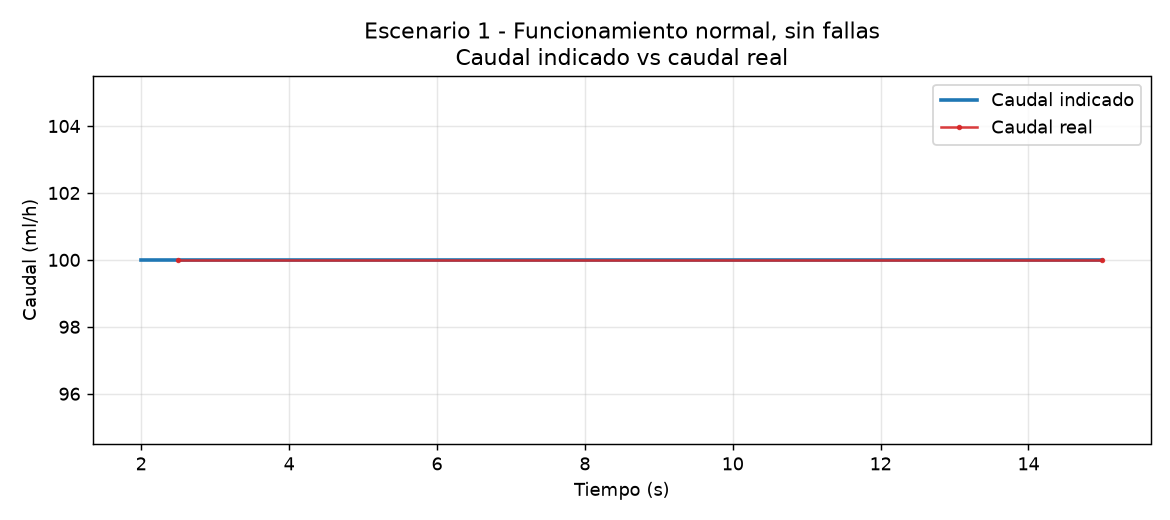
\includegraphics[width=0.82\textwidth]{graficos/escenario_1_funcionamiento_normal_sin_fallas/01_caudal_indicado_vs_real.png}
\caption{Escenario 1: el caudal real (rojo) sigue al indicado (azul) tras la latencia de 0,5~s y se mantiene en 100~ml/h.}
\label{fig:esc1}
\end{figure}

\paragraph{Escenario 5 --- desvío sostenido y alarma crítica.} Orden de 100~ml/h con \texttt{falla=0.5}: el actuador entrega 50~ml/h (desvío del 50\%).

\begin{lstlisting}[style=cml]
t=  2.00  evento  inicio_infusion
t=  2.50  caudal  50.0
t=  3.00  evento  correccion_caudal
t=  4.00  evento  correccion_caudal
t=  5.00  evento  correccion_caudal
t=  6.00  evento  correccion_caudal
t=  7.00  evento  correccion_caudal
t=  8.00  evento  desvio_sostenido
t=  8.00  alarma  media
t= 11.00  evento  critica_stop
t= 11.00  alarma  critica
t= 11.50  caudal  0.0
\end{lstlisting}

\noindent Las muestras 1--5 ($t=3$ a $7$~s) disparan \texttt{correccion\_caudal} sin éxito (el actuador sigue fallando); la sexta ($t=8$~s) alcanza \texttt{N\_MEDIA} y emite \texttt{alarmaMedia} (T2: 5~s desde el primer desvío). Las muestras 7 y 8 solo cuentan; la novena ($t=11$~s) alcanza \texttt{N\_CRITICA}, emite \texttt{alarmaCritica} y detiene la bomba, cuyo caudal real cae a 0 a los 11,5~s. La bomba no reanuda (S3). Pasan S2, S3, L1, T1 y T2.

\begin{figure}[H]
\centering
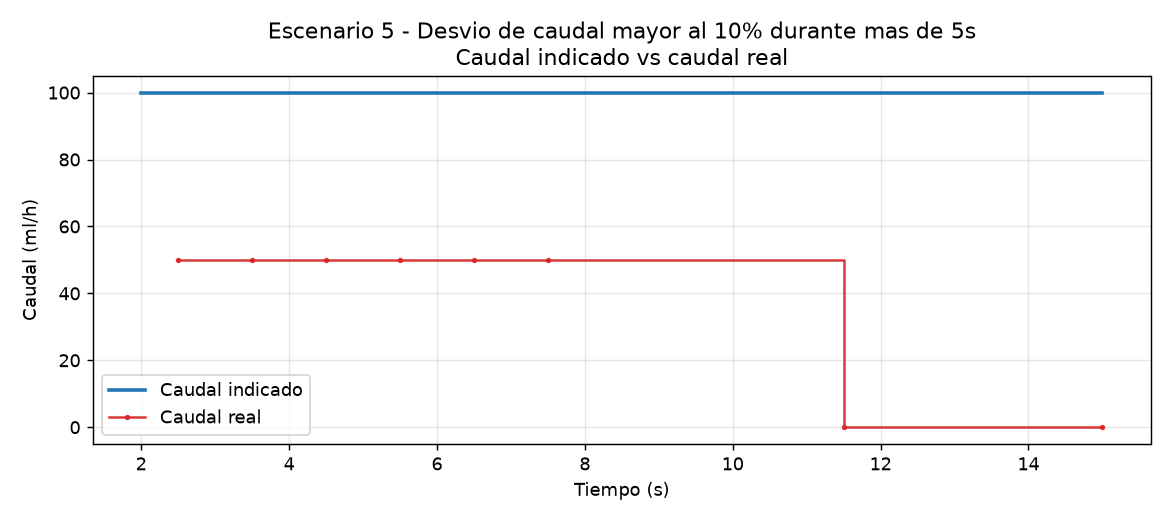
\includegraphics[width=0.8\textwidth]{graficos/escenario_5_desvio_de_caudal_mayor_al_10_durante_mas_de_5s/01_caudal_indicado_vs_real.png}\\[6pt]
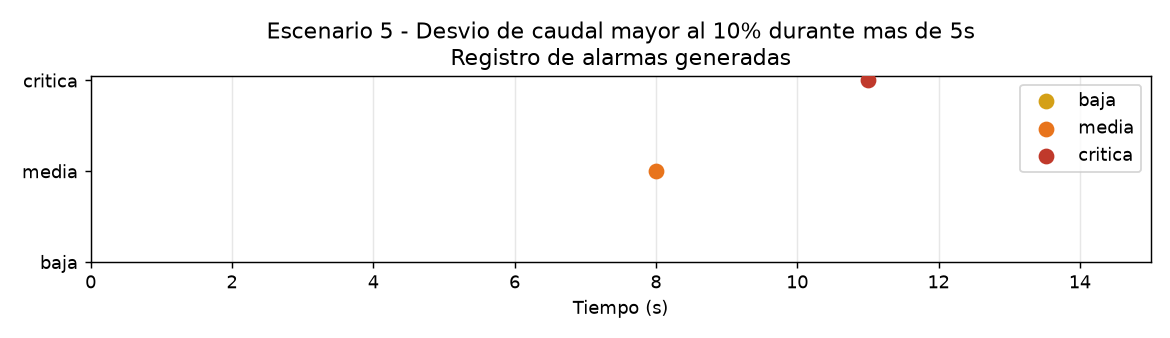
\includegraphics[width=0.8\textwidth]{graficos/escenario_5_desvio_de_caudal_mayor_al_10_durante_mas_de_5s/03_registro_alarmas.png}
\caption{Escenario 5. Arriba: el caudal real se queda en 50~ml/h (objetivo 100) hasta que la bomba se detiene. Abajo: la escalada de alarmas media~$\to$~crítica.}
\label{fig:esc5}
\end{figure}

\paragraph{Escenario 6 --- fin de bolsa con confirmación.} Orden de 100~ml/h; \texttt{finBolsa} a los 10~s y confirmación del enfermero a los 30~s.

\begin{lstlisting}[style=cml]
t=  2.00  evento  inicio_infusion
t=  2.50  caudal  100.0
t= 10.00  evento  fin_bolsa
t= 10.00  alarma  baja
t= 30.00  evento  reanudacion_post_bolsa
\end{lstlisting}

\noindent Al detectar \texttt{finBolsa} se emite \texttt{alarmaBaja} y el controlador entra en modo \texttt{bolsa} con la cuenta regresiva de 60~s; la infusión continúa mientras tanto. La confirmación a los 30~s (el enfermero repuso la bolsa) la reanuda antes del autostop: se emite \texttt{reanudacion\_post\_bolsa} y el modo vuelve a \texttt{infund} (figura~\ref{fig:esc6}). El fin de bolsa se resolvió en 20~s, dentro del límite de 60~s. Pasan S2, L1, L3, T1 y T3.

\begin{figure}[H]
\centering
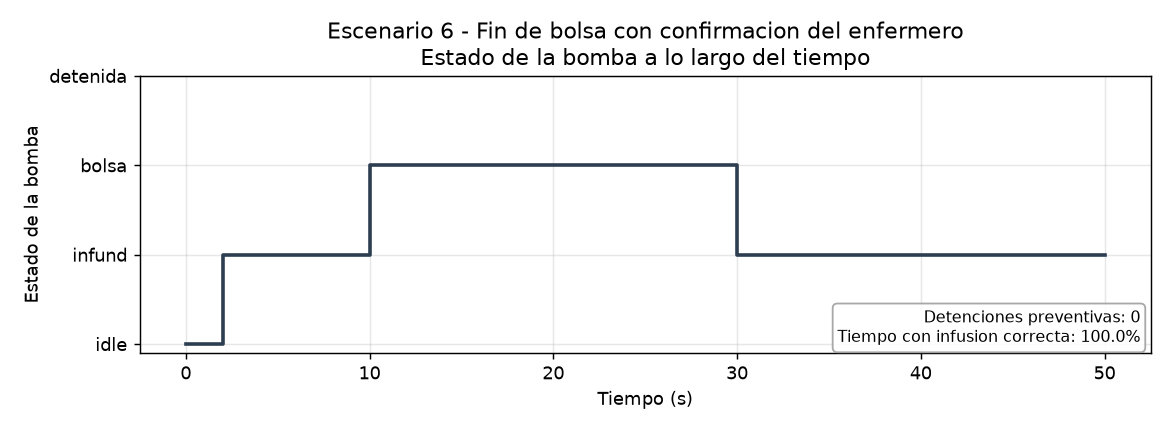
\includegraphics[width=0.8\textwidth]{graficos/escenario_6_fin_de_bolsa_con_confirmacion_del_enfermero/02_estado_bomba.png}\\[6pt]
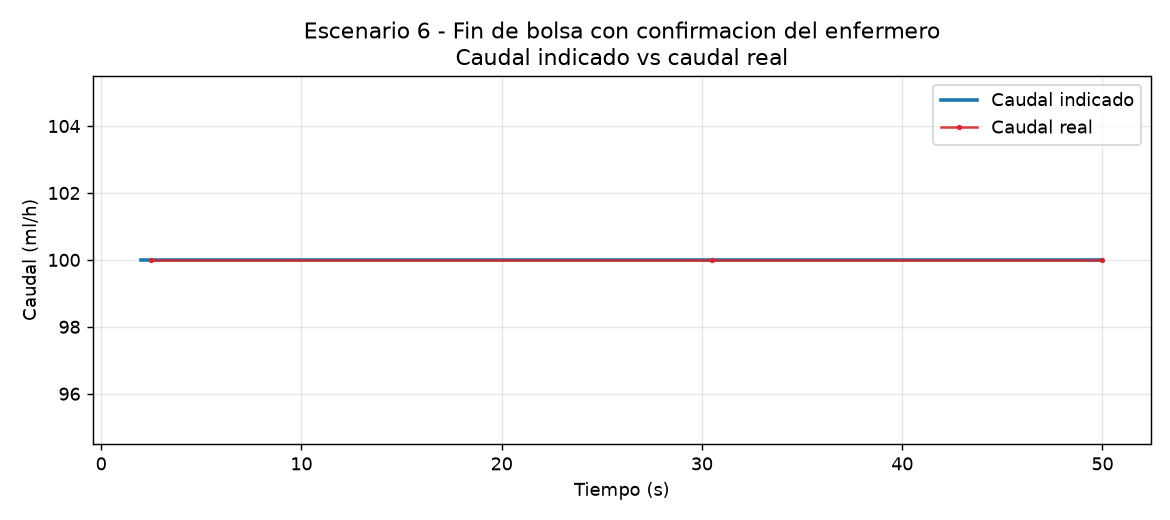
\includegraphics[width=0.8\textwidth]{graficos/escenario_6_fin_de_bolsa_con_confirmacion_del_enfermero/01_caudal_indicado_vs_real.png}
\caption{Escenario 6. Arriba: el estado pasa de \texttt{infund} a \texttt{bolsa} en $t=10$ y vuelve a \texttt{infund} en $t=30$ por la confirmación. Abajo: el caudal real no se interrumpe durante la ventana de bolsa.}
\label{fig:esc6}
\end{figure}

\paragraph{Escenario 7 --- alarma crítica no confirmada.} Mismo desvío que el escenario 5, pero sin confirmación y con horizonte de 62~s.

\begin{lstlisting}[style=cml]
t=  2.00  evento  inicio_infusion
t=  2.50  caudal  50.0
   (correcciones 1--5, alarmaMedia y critica_stop como en el escenario 5)
t= 11.00  alarma  critica
t= 41.00  alarma  critica
t= 51.00  alarma  critica
t= 61.00  alarma  critica
\end{lstlisting}

\noindent Tras la \texttt{alarmaCritica} inicial a los 11~s, al no confirmarse se repite a los 41~s (30~s después, \texttt{T\_CONF}) y luego cada 10~s (\texttt{T\_REP}): a los 51 y 61~s (figura~\ref{fig:esc7}). Es el único escenario que ejercita la repetición completa de la crítica: pasan S2, S3, L1, L2, T1, T2 y T4.

\begin{figure}[H]
\centering
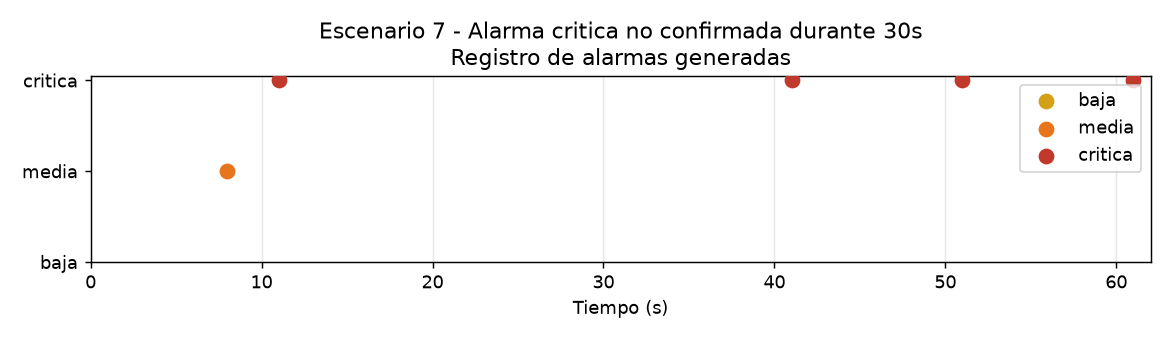
\includegraphics[width=0.8\textwidth]{graficos/escenario_7_alarma_critica_no_confirmada_durante_30s/03_registro_alarmas.png}
\caption{Escenario 7: la alarma crítica se repite a los 11, 41, 51 y 61~s (primera repetición a los 30~s, luego cada 10~s).}
\label{fig:esc7}
\end{figure}

\end{document}
